\chapter{Background}\label{Background}

This chapter offers an overview of the technology and concepts needed to understand the context and relevance of the work within the broader world. The review is conducted predominately through a networking, security and privacy perspective to best highlight the aspects pertinent to the distributed deployment of ECH. This chapter also represents the bulk of the effort put into investigating and studying the functioning of ECH while identifying and experimenting with different deployment models.

The contents of this chapter include a high level description of the Transport Layer Security protocol and the Domain Name System with a more detailed look at the components that enable ECH functionality. This is followed by an inspection of ECH itself, its security properties and the mechanisms which allow for distributed deployment. Finally, we survey how a variety of traffic analysis techniques that can be used to infer sensitive information from patterns in network activity, as well as the countermeasures which exist to mask these patterns.








\section{Transport Layer Security}

Transport Layer Security (TLS) is a cryptographic protocol proposed by the Internet Engineering Task Force (IETF) which enables secure network communication over public networks. Applications and services can establish an encrypted communication channel to transmit private information such that confidentiality, integrity and authenticity of the data can be ensured. TLS is commonly used to protect Internet traffic, having seen widespread adoption and several revisions since its original inception in 1999, superseding the Secure Sockets Layer (SSL) specification previously defined by Netscape Communications from 1994~\cite{chan2018monitoring, LE-HTTPS, rfc2246}.

TLS is designed to operate on top of a reliable transmission protocol between a client and server, such as the Transmission Control Protocol (TCP) when used over the Internet. In order to prevent eavesdropping, tampering and message forgery, TLS includes a number of security features based on a number of cryptographic mechanisms:

\begin{description}
\item[Confidentiality:] All service and application data exchanged between the client and server is encrypted as to make it indecipherable to any intermediate party which might be intercepting their communication. For example, consider the importance of protecting customer passwords and banking information when accessing financial services.
\item[Data integrity:] In a similar manner, cryptographic properties are used to guarantee transferred data cannot be modified during transmission. This is critical for safeguarding against input manipulation in consequential situations, such as while conducting a monetary transaction.
\item[Authentication:] TLS provides the ability for both participants to verify the identity of the other, ensuring privileged communication is only performed with the intended recipient. Such a condition is fundamental for establishing trust and confidence in sensitive environments, as is required when interacting with online financial institutions.
\end{description}

TLS 1.3 is the latest defined standard for the protocol, having been published in August 2018 and contributing to the deprecation of TLS 1.0 and TLS 1.1 in March 2021~\cite{rfc8446, rfc8996}. <deployment stats>. It introduces many major changes to TLS 1.2, including the addition of a zero round trip time resumption (0-RTT) mode, further encryption and optimisation of the handshake and removal of outdated cryptographic algorithms and security mechanism with all key exchanges now providing forward secrecy. A change of particular relevance to ECH is the encryption of the digital certificate received by the client to authenticate the server.

\subsection{Digital Certificates}

TLS uses digital certificates to make assertions on the identity of entities within the network using a chain of trust model, and are of particular significance during the exchange of public keys. <what public key used for> <"the TLS connection handshake would be susceptible to man-in-the-middle attacks"> <therefore trust must be established>

<chain of trust model is a hierarchical structure of certificates, Fig~\ref{tls_chain_figure}>
<ensures each certificate in the chain is issued by a trusted Certificate Authority (CA)>
<root ca is inherently trusted>
<These certificates contain public key, parent name, signature and other metadata>

\begin{figure}[ht]
\centerline{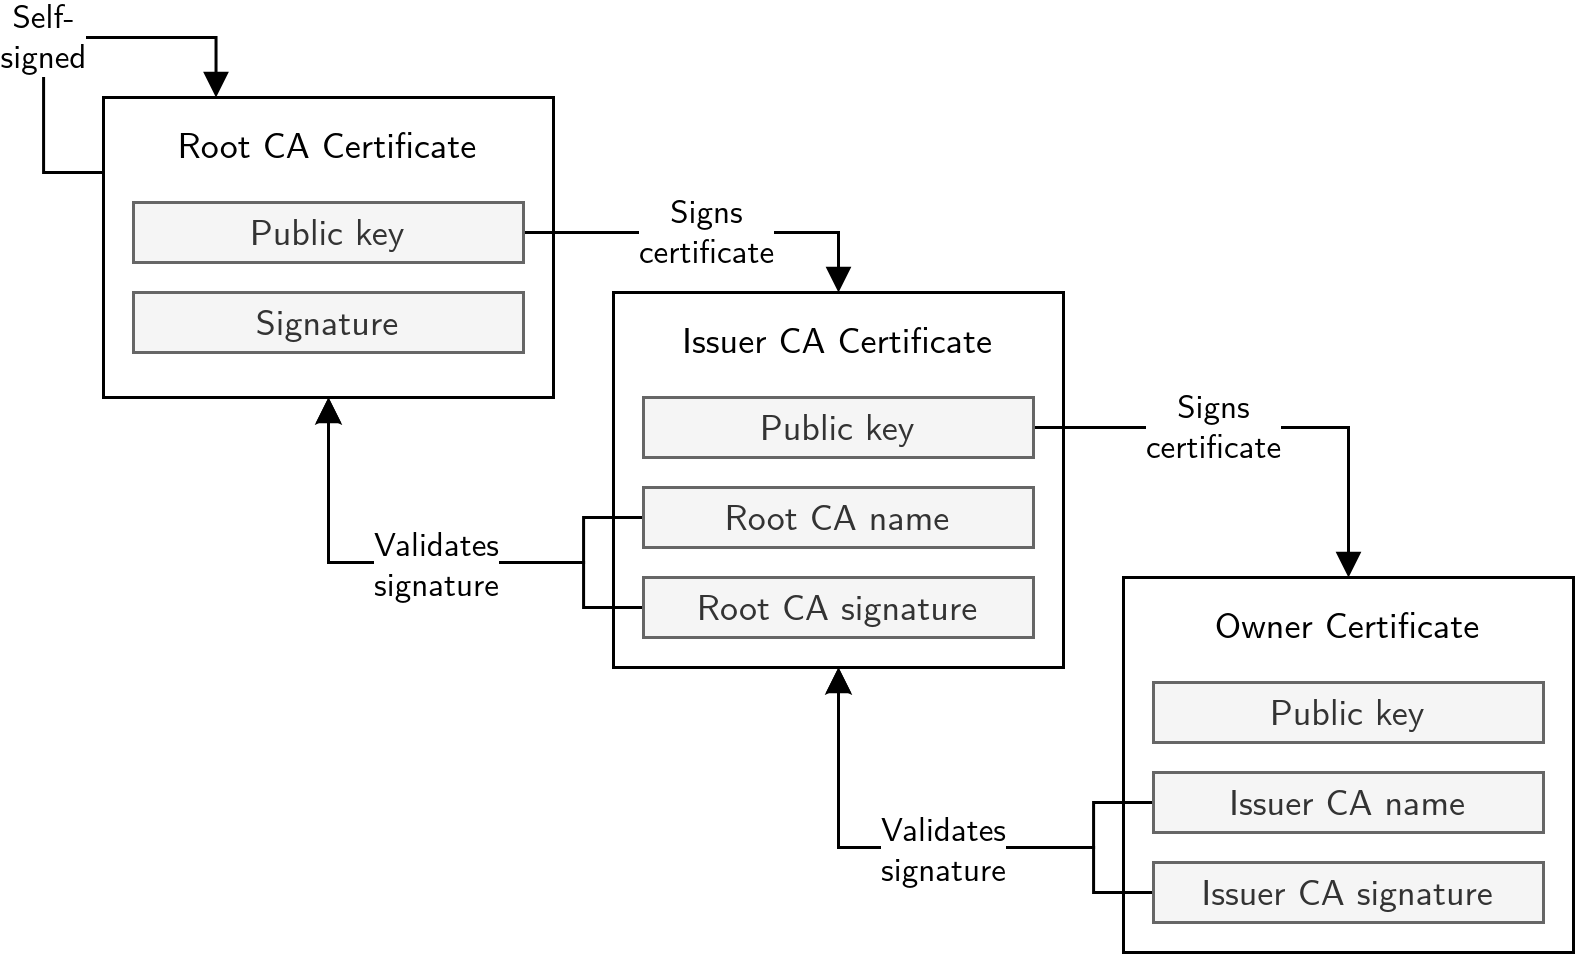
\includegraphics[width=160mm]{images/tls-chain.png}}
\caption[TLS certificate chain of trust]{<>}
\label{tls_chain_figure}
\end{figure}

<root ca typically installed by operating system>
<it is possible to add your own>
<typically only server is authenticated, it sends its cert and public key during the handshake>
<its certificate is verified by the client>

\subsection{TLS 1.3 Handshake}

<the tls handshake is a procedure executed between the client and server to complete establishment>
<tls 1.3 was designed to improve the security and performance of the handshake over 1.2 while reducing overall complexity>
<Fig.~\ref{tls_handshake_figure}>
<application data>

\begin{figure}[ht]
\centerline{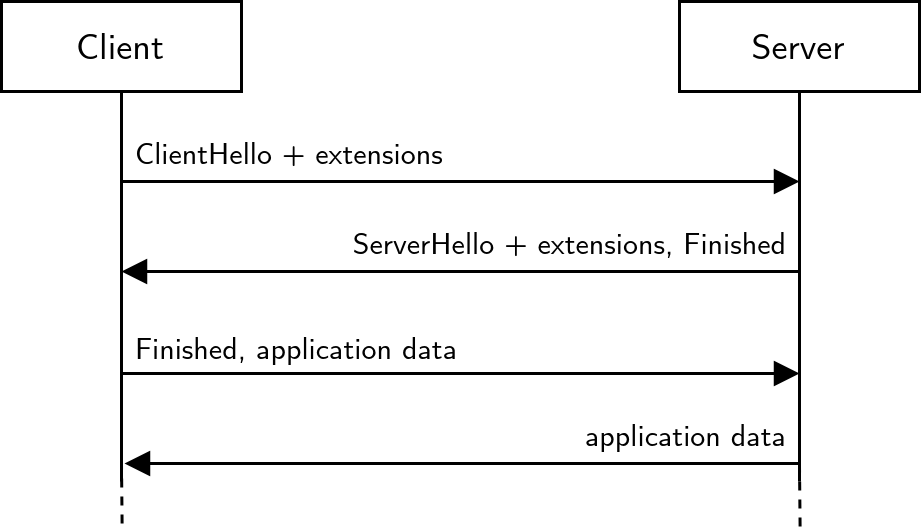
\includegraphics[width=120mm]{images/tls-handshake.png}}
\caption[Basic TLS 1.3 handshake]{<>}
\label{tls_handshake_figure}
\end{figure}

<The handshake consists of a number of required and optional messages with some plain and others encrypted:>

\begin{description}
\item[ClientHello:] <clienthello contents+purpose>
\item[ServerHello:] <serverhello contents+purpose>
\item[Certificate:] <optional certificate, now encrypted>
\item[Finished:] <finish protocol>
\end{description}

<in addition to these, the handshake offers extensions>

\subsection{Extensions}

<to remain adaptable, tls 1.3 permits numerous extensions to be inserted during the handshake for additional features and capabilities>
<some are mandatory in 1.3 and others are very commonly used>
<examples: ems, sni, alpn... and problems they solve>
<wider range of use cases and accommodating evolving requirements>
<examples: ech, ...>

<problems>
<greasing>








\section{The Domain Name System}

<history of ip, why dns needed>
<the domain name system (dns) was introduced to add alphanumeric domain names>
<originally a big host file>
<it now operates as a decentralised hierarchical naming system accessible by networked devices>
<registration consists of a number of entities registrars, registrants, registries>
<name server>

\subsection{Name Resolution Process}

<consists of root ns, tld ns, authoritative ns>
<Fig.~\ref{dns_resolve_figure}>
<stub resolver queries local recursive resolver>
<if not cached, asks root-tld-etc>

\begin{figure}[ht]
\centerline{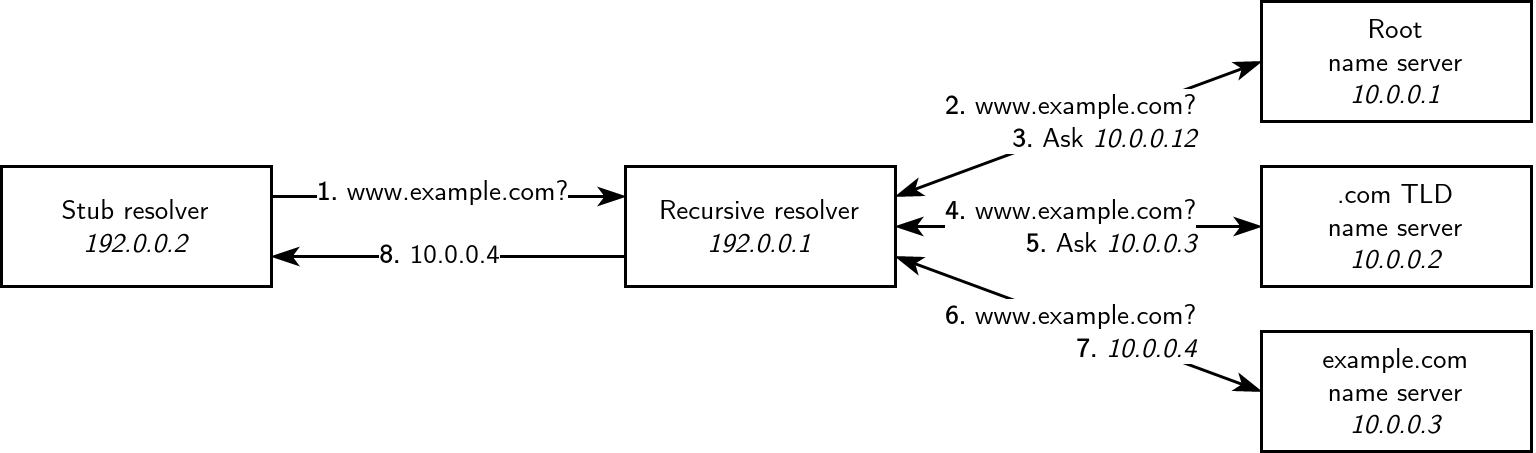
\includegraphics[width=160mm]{images/dns-resolve.png}}
\caption[Example DNS name resolution process]{<example dns query resolution process for www.example.com>}
\label{dns_resolve_figure}
\end{figure}

<dns protocol>

\subsection{DNS Over HTTPS}

<security was previously not a concern as the information was considered public>
<passive attacks considered bad \cite{todo}>
<introduction of dot>
<problems>
<introduction of doh>
<doh security>

\subsection{The HTTPS Resource Record}

<these days a number of resource records exist for more advanced functionality and adaptability>
<new rr have been added to support performace and some fixes\cite{https-rr}>
<this has also allowed additional data to be accociated with a host>
<ech uses this as the primary mechanism to transmit echconfig out-of-band to clients>








\section{Encrypted Client Hello}

<why need ech>
<what ech is "Encrypted Client Hello (ECH) is a proposed extension for TLS 1.3 which has begun to see implementation and adoption on the Internet~\cite{tsiatsikas2022measuring, CF-ECH}">
<what ech does "ECH seeks to allow encryption of the ClientHello message, which can contain potentially sensitive information such as the Service Name Indication (SNI) and Application-Layer Protocol Negotiation (ALPN) extensions."
<how ech does this "This is partially achieved through serving many private domains behind a common provider to form an anonymity set that conceals the true domain requested by the client.">

The client-facing server first generates an ECH encryption key pair and some associated metadata. This public key and metadata, referred to as an ECH configuration or ECHConfig, may then be shared out-of-band to ECH-enabled clients though secure means like DoH. A client may then use this to construct a ClientHello message, named the ClientHelloOuter, holding unremarkable values for the client-facing server along side an encrypted ClientHello, named the ClientHelloInner, itself holding the real values for a private domain. To establish a TLS connection to the origin server of this domain, the client sends the ClientHelloOuter to the client-facing server, which decrypts and relays the contained ClientHelloInner to the origin server, which itself completes the TLS handshake with the client through the client-facing server.

<in this way, the true domain is concealed>

\subsection{Hybrid Public Key Encryption}

<much like tls itself, the ech extension uses public key cryptography>
<shown to be secure>\cite{bhargavan2022symbolic}
<HPKE explanation>

\subsection{Split Mode Deployment}

<ech defines two modes of network topology>
<shared mode is when the client-facing server and backend server are co-located, and is not of interest to us>
<split mode is when the client-facing server and backend server are in different boxes pysically separateed>
<Fig.~\ref{ech_split_mode_figure}>

\begin{figure}[ht]
\centerline{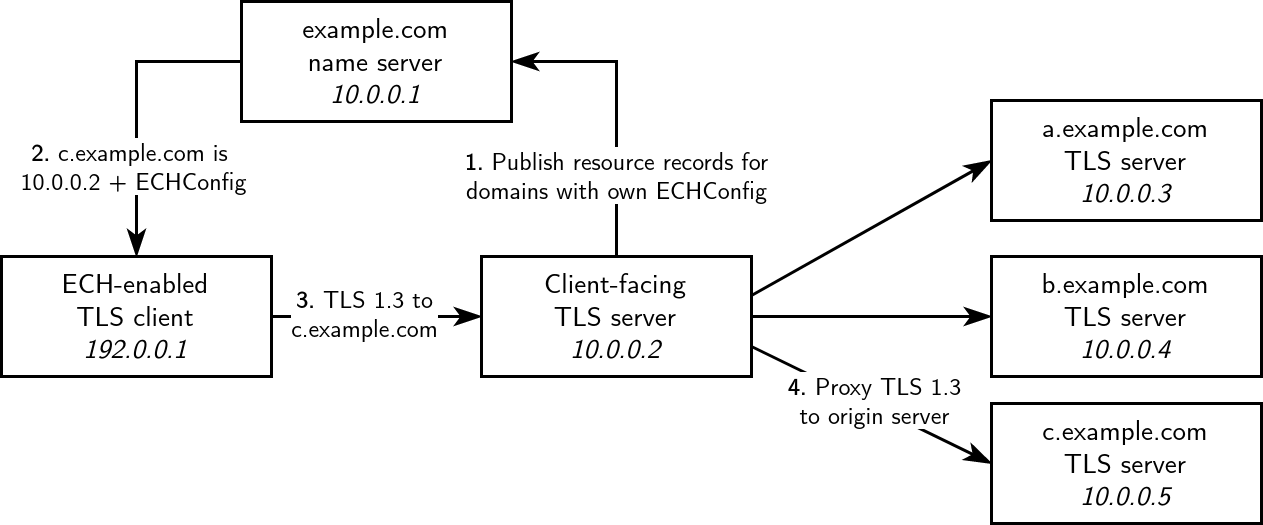
\includegraphics[width=160mm]{images/ech-split-mode.png}}
\caption[Example ECH Split Mode deployment]{<>}
\label{ech_split_mode_figure}
\end{figure}

<this is useful for x,y,z...>
<distributed deployment explanation (as opposed to centralised and decentralised)>
<however it is susceptible to attacks>







\section{Traffic Analysis}

<what is traffic analysis>
<traffic analysis techniques that can be used to infer sensitive information from patterns in network activity>
<exploits information unintentionally leaked by the system aka side-channel attack>
<example of the act of communication being information itself>
<there are a lot of other techniques that can be used: packet inspection>

\subsection{Correlation Attacks}

<is a large category of attacks identified by correlating communication patterns>
<can be used to break anonymity, very relevant to ech split mode>
<examples: timing, packet size, packet count, packet rate+pattern>

\subsection{Countermeasures}

<to disrupt the patterns>
<effectiveness against practicality>
<examples: morphing, mixing/pacing and padding, normalisation>








\section{Summary}

<tls and dns continue to evolve with shifting requirements>
<ech has been enabled due to this, which allows for the encryption of the clienthello>
<ech split mode permits the client-facing server to be pysically separate from the backend server>
<this reveals potentially attack surface through traffic correlation, which must be distributed with various countermeasures>
